 \subsection{PRISM}
 PRISM is a probabilistic model checker allowing formal modelling and analysis of systems that exhibit random or probabilistic behaviour. In our case, we will use PRISM to model a Continuous-Time Markov Chain (CTMCs) but there are other models that can be be modeled thanks to this tool. \\
 Thanks to PRISM, we will for example be able to show that every traffic lights will get the green light in an equal and fair way, meaning that there will be no starvation for one of them. Moreover, thanks to PRISM, we can show the statistics of green light possession for every different traffic light, something that is not possible to do in Uppaal. This is why we decided to also rewrite our model in PRISM so new kind of properties could be demonstrated.
 \begin{figure}[h]\label{fig:prism}
  \begin{center}
    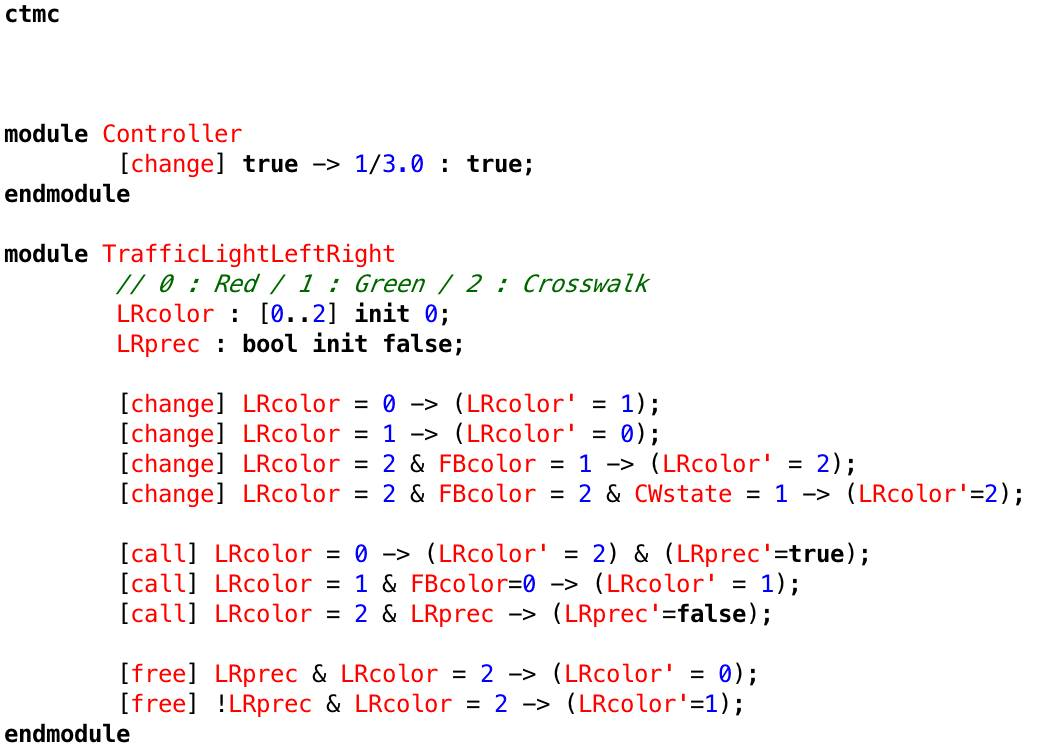
\includegraphics[width=0.8\textwidth]{picture/prism.png}
    \caption{Example of the PRISM language}
  \end{center}
\end{figure} 
bla

